\documentclass{beamer}
%\documentclass[handout]{beamer}
\usetheme{Antibes}

\usepackage{fontspec}
\usepackage[catalan]{babel}
\usepackage{hyperref}
\usepackage[normalem]{ulem}
\usepackage{tikz}
\usepackage{listings}

\newcommand*{\framemargin}{3ex}
\newcommand*{\literatecolour}{\textcolor{literatecolour}}
\newcommand*{\pythonprompt}{\textcolor{promptcolour}{{>}{>}{>}}}

\definecolor{gray}{gray}{0.5}
\colorlet{commentcolour}{green!50!black}
\colorlet{stringcolour}{red!60!black}
\colorlet{keywordcolour}{magenta!90!black}
\colorlet{exceptioncolour}{yellow!50!red}
\colorlet{commandcolour}{blue!60!black}
\colorlet{numpycolour}{blue!60!green}
\colorlet{literatecolour}{magenta!90!black}
\colorlet{promptcolour}{green!50!black}
\colorlet{specmethodcolour}{violet}

\lstdefinestyle{mypython}{
	numbers=left,
	language=python,
	showtabs=true,
	tab=,
	tabsize=2,
	basicstyle=\ttfamily\footnotesize,%\setstretch{.5},
	stringstyle=\color{stringcolour},
	showstringspaces=false,
	alsoletter={1234567890},
	otherkeywords={\%, \}, \{, \&, \|},
	keywordstyle=\color{keywordcolour}\bfseries,
	emph={and,break,class,continue,def,yield,del,elif ,else,%
		except,exec,finally,for,from,global,if,import,in,%
		lambda,not,or,pass,print,raise,return,try,while,assert,with},
	emphstyle=\color{blue}\bfseries,
	emph={[2]True, False, None},
	emphstyle=[2]\color{keywordcolour},
	emph={[3]object,type,isinstance,copy,deepcopy,zip,enumerate,reversed,list,set,len,dict,tuple,xrange,append,execfile,real,imag,reduce,str,repr},
	emphstyle=[3]\color{commandcolour},
	emph={Exception,NameError,IndexError,SyntaxError,TypeError,ValueError,OverflowError,ZeroDivisionError},
	emphstyle=\color{exceptioncolour}\bfseries,
	morecomment=[s]{"""}{"""},
	commentstyle=\color{commentcolour}\slshape,
	emph={[4]ode, fsolve, sqrt, exp, sin, cos,arctan, arctan2, arccos, pi,  array, norm, solve, dot, arange, isscalar, max, sum, flatten, shape, reshape, find, any, all, abs, plot, linspace, legend, quad, polyval,polyfit, hstack, concatenate,vstack,column_stack,empty,zeros,ones,rand,vander,grid,pcolor,eig,eigs,eigvals,svd,qr,tan,det,logspace,roll,min,mean,cumsum,cumprod,diff,vectorize,lstsq,cla,eye,xlabel,ylabel,squeeze},
	emphstyle=[4]\color{numpycolour},
	emph={[5]__init__,__add__,__mul__,__div__,__sub__,__call__,__getitem__,__setitem__,__eq__,__ne__,__nonzero__,__rmul__,__radd__,__repr__,__str__,__get__,__truediv__,__pow__,__name__,__future__,__all__},
	emphstyle=[5]\color{specmethodcolour},
	emph={[6]assert,yield},
	emphstyle=[6]\color{keywordcolour}\bfseries,
	emph={[7]range},
	emphstyle={[7]\color{keywordcolour}\bfseries},
	literate=*%
	{:}{{\literatecolour:}}{1}%
	{=}{{\literatecolour=}}{1}%
	{-}{{\literatecolour-}}{1}%
	{+}{{\literatecolour+}}{1}%
	{*}{{\literatecolour*}}{1}%
	{**}{{\literatecolour{**}}}2%
	{/}{{\literatecolour/}}{1}%
	{//}{{\literatecolour{//}}}2%
	{!}{{\literatecolour!}}{1}%
	%{(}{{\literatecolour(}}{1}%
	%{)}{{\literatecolour)}}{1}%
	{[}{{\literatecolour[}}{1}%
	{]}{{\literatecolour]}}{1}%
	{<}{{\literatecolour<}}{1}%
	{>}{{\literatecolour>}}{1}%
	{>>>}{\pythonprompt}{3}%
	,
	rulecolor=\color{black!40},
	backgroundcolor=\color{white},
	breakindent=.5\textwidth,frame=single,breaklines=true,
}



\AtBeginSection[]
{
	\begin{frame}{Contingut}
		\tableofcontents[currentsection]
	\end{frame}
}

\title{Construcció d'una orquestra amb Raspberry Pi}
\author{Arnau Canyadell Miquel \and Joan Marcè Igual}
\date{2 de Juny de 2017}

\begin{document}

\frame{\titlepage}
\section{Introducció}
\begin{frame}{Descripció del projecte}
	Crear amb Raspberry Pi una orquestra musical formada per un director i uns quants músics que interpreten el que els mana el director.
	\begin{figure}
		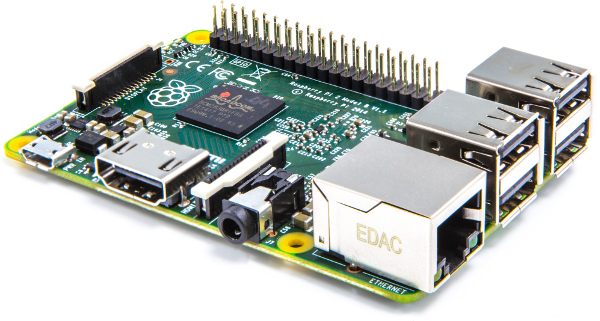
\includegraphics[width=0.475\linewidth]{images/raspberry}
		\hfill
		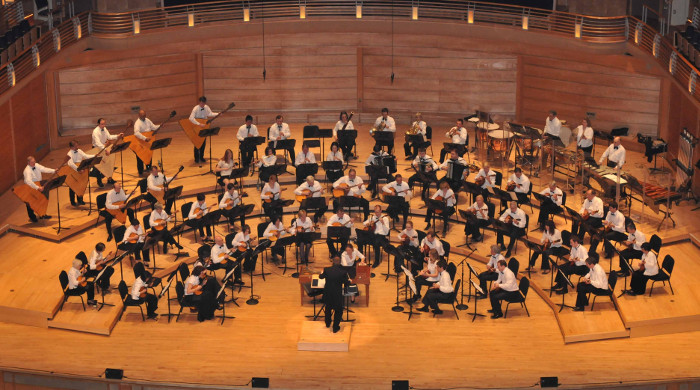
\includegraphics[width=0.475\linewidth]{images/orchestra}
	\end{figure}
\end{frame}

\section{Objectius}
\subsection{Objectius a curt termini}
\begin{frame}{Objectius a curt termini}
	
	\begin{itemize}
		\item Aconseguir rebre la música d'un ordinador
		\item Enviar la música a una Raspberry Pi
		\item Reproduir la música en una Raspberry Pi
	\end{itemize}
\end{frame}

\subsection{Objectius a llarg termini}
\begin{frame}{Objectius a llarg termini}
	\begin{itemize}
		\item Programar un bot per a l'aplicació de missatgeria Telegram que reprodueixi amb l'orquestra de Raspberry Pis la música que se li enviï.
		\item Enviar música del mòbil a l'ordinador.
	\end{itemize}
\end{frame}

\section{Feina feta}
\begin{frame}{Què hem fet fins ara?}
	\begin{itemize}
		\item Establiment dels objectius
		\item Analitzat el codi del director
		\item Programat el codi de l'intèrpret (músic)
		\item Codi per configurar una raspberry pi qualsevol per a funcionar com a músic
		\item Canvis en el codi del director
	\end{itemize}
\end{frame}

\begin{frame}
	\frametitle{Principals problemes trobats i solucionats}
	\begin{itemize}[<+->]
		\item Mida de les targetes SD. 4 GB no era suficient.
		\begin{itemize}
			\item Usar una targeta més gran
			\item Usar versió LITE de \texttt{Raspbian}
		\end{itemize}
		\item Àudio en la raspberry pi. No hem sabut canviar el dispositiu de sortida des de l'entorn de comandes. Hem hagut d'insta\l.lar l'entorn gràfic a la raspberry pi.
		\begin{itemize}
			\item Finalment trobat
			\item Crear script que canvii el dispositiu per defecte
		\end{itemize}
		\item La llibreria midi Music21 és molt lenta per llegir midi.
		\begin{itemize}
			\item Usar la llibreria \texttt{mido}.
		\end{itemize}
	\end{itemize}
\end{frame}

\section{Funcionament}
\subsection{Multicast}
\begin{frame}{Multicast}
	\begin{figure}[H]
	\centering
	\def\width{.1\textwidth}
	\begin{tikzpicture}
		\node[
			label = left:{Router}]
			(router){
\includegraphics[width=\width]{images/cisco/router}};
		\node[
			below = of router, 
			label = left:{Switch}] 
			(switch){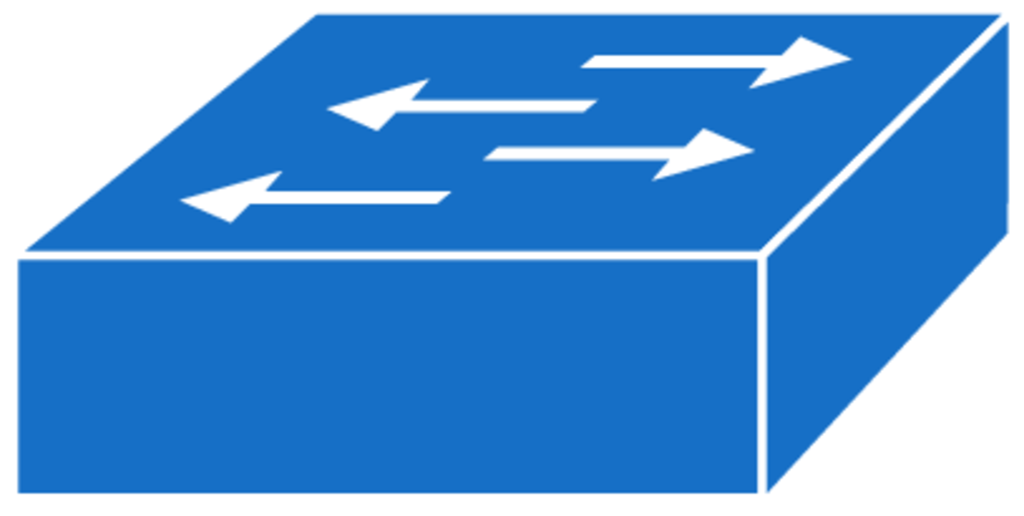
\includegraphics[width=\width]{images/cisco/workgroup_switch} };
		\node[
			below left = of switch,
			label = below:{Director}]
			(director){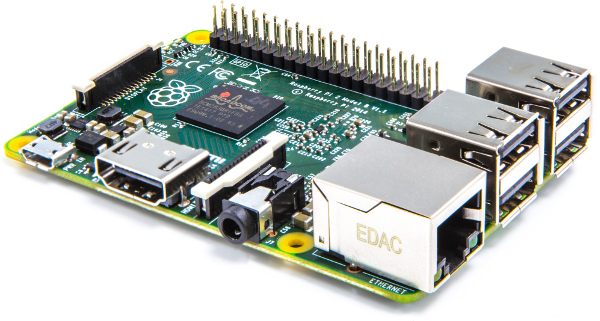
\includegraphics[width=\width]{images/raspberry}};
		\node[
			below right = of switch,
			label = below:{Músic 1}]
			(m1){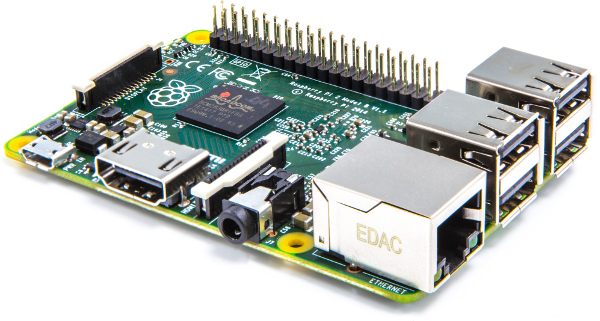
\includegraphics[width=\width]{images/raspberry}};
		\node[
			right = of m1,
			label = below:{Músic 2}]
			(m2){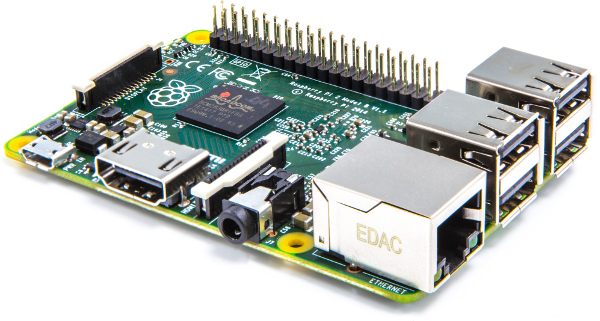
\includegraphics[width=\width]{images/raspberry}};
		\node[
			right = of m2,
			label = below:{Músic 3}]
			(m3){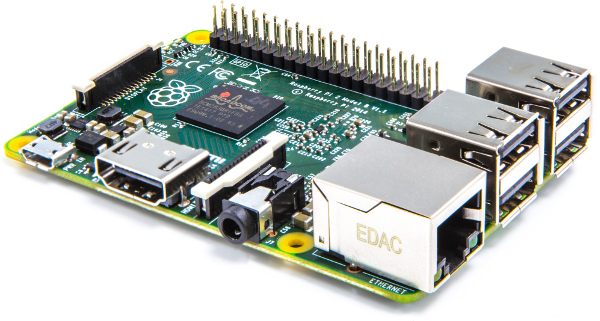
\includegraphics[width=\width]{images/raspberry}};	
		
		\draw[latex-latex] (router) -- (switch);
		\draw[-latex] (director) -- (switch);
		\draw[-latex] (switch) -- (m1);
		\draw[-latex] (switch) -- (m2);
		\draw[-latex] (switch) -- (m3);
	\end{tikzpicture}
	\caption{Esquema de funcionament de la xarxa}
\end{figure}
\end{frame}
\subsection{Bucle reproducció}
\begin{frame}[fragile]{Bucle de reproducció}
	\begin{lstlisting}[
			label={lst:code},
			style=mypython, 
			basicstyle=\ttfamily\tiny,
			captionpos=b,
			xleftmargin=.05\textwidth, 
			xrightmargin=.05\textwidth,
			caption={Bucle bàsic per enviar les dades de notes}
		]
	# file_path: conté el camí fins a l'arxiu
	# multicast_group: conté la ip al grup de multicast
	# La funció play_tracks() ja fa les pauses que s'hagin de fer perquè
	# les notes sonin quan toca
	mid = DirectorMidiFile(file_path)
	for missatge, track in mid.play_tracks():
		msg_in, msg_out = descodifica(missatge, track)
		# Genera string a enviar
		json_string = json.dumps({
		"in": msg_in,
		"out": msg_out
		})
		
		# Enviar dades al multicast
		socket.sendto(json_string.encode(), multicast_group)
	\end{lstlisting}
\end{frame}

\section{Demostració}
\begin{frame}{Demostració en directe}
	\begin{figure}
		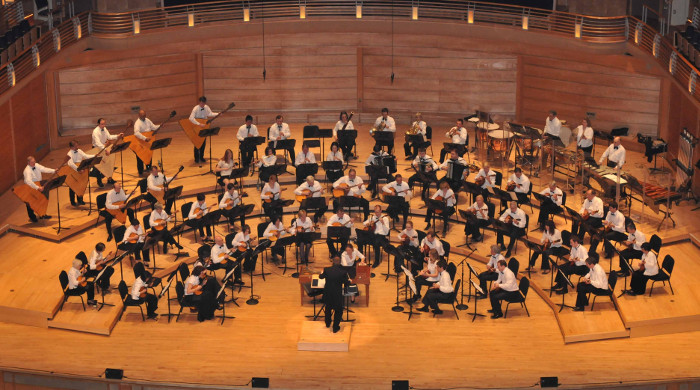
\includegraphics[width=\linewidth]{images/orchestra}
	\end{figure}
\end{frame}

\end{document}